% Options for packages loaded elsewhere
% Options for packages loaded elsewhere
\PassOptionsToPackage{unicode}{hyperref}
\PassOptionsToPackage{hyphens}{url}
%
\documentclass[
  ngerman,
  10pt,
  letterpaper,
]{book}
\usepackage{xcolor}
\usepackage[top=2.5cm,bottom=2.5cm,left=2.5cm,right=2.5cm]{geometry}
\usepackage{amsmath,amssymb}
\setcounter{secnumdepth}{5}
\usepackage{iftex}
\ifPDFTeX
  \usepackage[T1]{fontenc}
  \usepackage[utf8]{inputenc}
  \usepackage{textcomp} % provide euro and other symbols
\else % if luatex or xetex
  \usepackage{unicode-math} % this also loads fontspec
  \defaultfontfeatures{Scale=MatchLowercase}
  \defaultfontfeatures[\rmfamily]{Ligatures=TeX,Scale=1}
\fi
\usepackage{lmodern}
\ifPDFTeX\else
  % xetex/luatex font selection
\fi
% Use upquote if available, for straight quotes in verbatim environments
\IfFileExists{upquote.sty}{\usepackage{upquote}}{}
\IfFileExists{microtype.sty}{% use microtype if available
  \usepackage[]{microtype}
  \UseMicrotypeSet[protrusion]{basicmath} % disable protrusion for tt fonts
}{}
\usepackage{setspace}
\makeatletter
\@ifundefined{KOMAClassName}{% if non-KOMA class
  \IfFileExists{parskip.sty}{%
    \usepackage{parskip}
  }{% else
    \setlength{\parindent}{0pt}
    \setlength{\parskip}{6pt plus 2pt minus 1pt}}
}{% if KOMA class
  \KOMAoptions{parskip=half}}
\makeatother
% Make \paragraph and \subparagraph free-standing
\makeatletter
\ifx\paragraph\undefined\else
  \let\oldparagraph\paragraph
  \renewcommand{\paragraph}{
    \@ifstar
      \xxxParagraphStar
      \xxxParagraphNoStar
  }
  \newcommand{\xxxParagraphStar}[1]{\oldparagraph*{#1}\mbox{}}
  \newcommand{\xxxParagraphNoStar}[1]{\oldparagraph{#1}\mbox{}}
\fi
\ifx\subparagraph\undefined\else
  \let\oldsubparagraph\subparagraph
  \renewcommand{\subparagraph}{
    \@ifstar
      \xxxSubParagraphStar
      \xxxSubParagraphNoStar
  }
  \newcommand{\xxxSubParagraphStar}[1]{\oldsubparagraph*{#1}\mbox{}}
  \newcommand{\xxxSubParagraphNoStar}[1]{\oldsubparagraph{#1}\mbox{}}
\fi
\makeatother

\usepackage{color}
\usepackage{fancyvrb}
\newcommand{\VerbBar}{|}
\newcommand{\VERB}{\Verb[commandchars=\\\{\}]}
\DefineVerbatimEnvironment{Highlighting}{Verbatim}{commandchars=\\\{\}}
% Add ',fontsize=\small' for more characters per line
\usepackage{framed}
\definecolor{shadecolor}{RGB}{241,243,245}
\newenvironment{Shaded}{\begin{snugshade}}{\end{snugshade}}
\newcommand{\AlertTok}[1]{\textcolor[rgb]{0.68,0.00,0.00}{#1}}
\newcommand{\AnnotationTok}[1]{\textcolor[rgb]{0.37,0.37,0.37}{#1}}
\newcommand{\AttributeTok}[1]{\textcolor[rgb]{0.40,0.45,0.13}{#1}}
\newcommand{\BaseNTok}[1]{\textcolor[rgb]{0.68,0.00,0.00}{#1}}
\newcommand{\BuiltInTok}[1]{\textcolor[rgb]{0.00,0.23,0.31}{#1}}
\newcommand{\CharTok}[1]{\textcolor[rgb]{0.13,0.47,0.30}{#1}}
\newcommand{\CommentTok}[1]{\textcolor[rgb]{0.37,0.37,0.37}{#1}}
\newcommand{\CommentVarTok}[1]{\textcolor[rgb]{0.37,0.37,0.37}{\textit{#1}}}
\newcommand{\ConstantTok}[1]{\textcolor[rgb]{0.56,0.35,0.01}{#1}}
\newcommand{\ControlFlowTok}[1]{\textcolor[rgb]{0.00,0.23,0.31}{\textbf{#1}}}
\newcommand{\DataTypeTok}[1]{\textcolor[rgb]{0.68,0.00,0.00}{#1}}
\newcommand{\DecValTok}[1]{\textcolor[rgb]{0.68,0.00,0.00}{#1}}
\newcommand{\DocumentationTok}[1]{\textcolor[rgb]{0.37,0.37,0.37}{\textit{#1}}}
\newcommand{\ErrorTok}[1]{\textcolor[rgb]{0.68,0.00,0.00}{#1}}
\newcommand{\ExtensionTok}[1]{\textcolor[rgb]{0.00,0.23,0.31}{#1}}
\newcommand{\FloatTok}[1]{\textcolor[rgb]{0.68,0.00,0.00}{#1}}
\newcommand{\FunctionTok}[1]{\textcolor[rgb]{0.28,0.35,0.67}{#1}}
\newcommand{\ImportTok}[1]{\textcolor[rgb]{0.00,0.46,0.62}{#1}}
\newcommand{\InformationTok}[1]{\textcolor[rgb]{0.37,0.37,0.37}{#1}}
\newcommand{\KeywordTok}[1]{\textcolor[rgb]{0.00,0.23,0.31}{\textbf{#1}}}
\newcommand{\NormalTok}[1]{\textcolor[rgb]{0.00,0.23,0.31}{#1}}
\newcommand{\OperatorTok}[1]{\textcolor[rgb]{0.37,0.37,0.37}{#1}}
\newcommand{\OtherTok}[1]{\textcolor[rgb]{0.00,0.23,0.31}{#1}}
\newcommand{\PreprocessorTok}[1]{\textcolor[rgb]{0.68,0.00,0.00}{#1}}
\newcommand{\RegionMarkerTok}[1]{\textcolor[rgb]{0.00,0.23,0.31}{#1}}
\newcommand{\SpecialCharTok}[1]{\textcolor[rgb]{0.37,0.37,0.37}{#1}}
\newcommand{\SpecialStringTok}[1]{\textcolor[rgb]{0.13,0.47,0.30}{#1}}
\newcommand{\StringTok}[1]{\textcolor[rgb]{0.13,0.47,0.30}{#1}}
\newcommand{\VariableTok}[1]{\textcolor[rgb]{0.07,0.07,0.07}{#1}}
\newcommand{\VerbatimStringTok}[1]{\textcolor[rgb]{0.13,0.47,0.30}{#1}}
\newcommand{\WarningTok}[1]{\textcolor[rgb]{0.37,0.37,0.37}{\textit{#1}}}

\usepackage{longtable,booktabs,array}
\usepackage{calc} % for calculating minipage widths
% Correct order of tables after \paragraph or \subparagraph
\usepackage{etoolbox}
\makeatletter
\patchcmd\longtable{\par}{\if@noskipsec\mbox{}\fi\par}{}{}
\makeatother
% Allow footnotes in longtable head/foot
\IfFileExists{footnotehyper.sty}{\usepackage{footnotehyper}}{\usepackage{footnote}}
\makesavenoteenv{longtable}
\usepackage{graphicx}
\makeatletter
\newsavebox\pandoc@box
\newcommand*\pandocbounded[1]{% scales image to fit in text height/width
  \sbox\pandoc@box{#1}%
  \Gscale@div\@tempa{\textheight}{\dimexpr\ht\pandoc@box+\dp\pandoc@box\relax}%
  \Gscale@div\@tempb{\linewidth}{\wd\pandoc@box}%
  \ifdim\@tempb\p@<\@tempa\p@\let\@tempa\@tempb\fi% select the smaller of both
  \ifdim\@tempa\p@<\p@\scalebox{\@tempa}{\usebox\pandoc@box}%
  \else\usebox{\pandoc@box}%
  \fi%
}
% Set default figure placement to htbp
\def\fps@figure{htbp}
\makeatother



\ifLuaTeX
\usepackage[bidi=basic]{babel}
\else
\usepackage[bidi=default]{babel}
\fi
% get rid of language-specific shorthands (see #6817):
\let\LanguageShortHands\languageshorthands
\def\languageshorthands#1{}
\ifLuaTeX
  \usepackage[german]{selnolig} % disable illegal ligatures
\fi


\setlength{\emergencystretch}{3em} % prevent overfull lines

\providecommand{\tightlist}{%
  \setlength{\itemsep}{0pt}\setlength{\parskip}{0pt}}



 
\usepackage[style=authoryear,backend=biber,style=authoryear-comp,uniquename=false,uniquelist=false]{biblatex}
\addbibresource{references.bib}


\usepackage{csquotes}
\usepackage{booktabs}
\usepackage{array}
\usepackage{multirow}
\usepackage{wrapfig}
\usepackage{float}
\usepackage{colortbl}
\usepackage{pdflscape}
\usepackage{threeparttable}
\usepackage{threeparttablex}
\usepackage[normalem]{ulem}
\usepackage{makecell}
\usepackage{xcolor}
\usepackage{multicol}
\usepackage{fancyhdr}
\usepackage{titlesec}
\usepackage{etoolbox}
\usepackage{tabularx}

% Define WISTA colors (brighter blue)
\definecolor{wistaBlue}{RGB}{30,110,180}
\definecolor{wistaLightBlue}{RGB}{51,153,204}
\definecolor{wistaDarkGray}{RGB}{64,64,64}
\definecolor{wistaLightGray}{RGB}{128,128,128}

% Custom section formatting for WISTA style
% Format: Number | Blue line | Dark gray title | Blue line
\titleformat{\section}
  {\color{wistaDarkGray}\Large\bfseries}
  {\color{wistaBlue}\Large\bfseries\thesection}
  {0.5em}
  {\color{wistaDarkGray}\Large\bfseries}
  [\vspace{0.2cm}\noindent{\color{wistaBlue}\rule{\columnwidth}{1.5pt}}\vspace{0.3cm}]

\titleformat{\subsection}
  {\color{wistaDarkGray}\large\bfseries}
  {\color{wistaBlue}\large\bfseries\thesubsection}
  {0.5em}
  {\color{wistaDarkGray}\large\bfseries}
  [\vspace{0.1cm}\noindent{\color{wistaBlue}\rule{\columnwidth}{1pt}}\vspace{0.2cm}]

% Header and footer setup
\pagestyle{fancy}
\fancyhf{} % Clear all header and footer fields
\fancyhead[LE]{\small\textit{Max Mustermann, Dr. Anna Schmidt}}
\fancyhead[RO]{\small\textit{Effizienzanalyse statistischer Verfahren}}
\fancyfoot[LE]{\small\thepage}
\fancyfoot[RE]{\small Statistisches Bundesamt | WISTA | {\color{wistaBlue}6} | 2025}
\fancyfoot[LO]{\small Statistisches Bundesamt | WISTA | {\color{wistaBlue}6} | 2025}
\fancyfoot[RO]{\small\thepage}
\renewcommand{\headrulewidth}{0pt}
\renewcommand{\footrulewidth}{0pt}

% Set up multicol parameters
\setlength{\columnsep}{1cm}
\setlength{\columnseprule}{0pt}

% Start two-column layout after title
\AtBeginDocument{
  \begin{multicols}{2}
}

% End two-column layout before end
\AtEndDocument{
  \end{multicols}
}

% Environment for full-width content
\newenvironment{fullwidth}{
  \end{multicols}
  \vspace{0.5cm}
}{
  \vspace{0.5cm}
  \begin{multicols}{2}
}
\makeatletter
\@ifpackageloaded{bookmark}{}{\usepackage{bookmark}}
\makeatother
\makeatletter
\@ifpackageloaded{caption}{}{\usepackage{caption}}
\AtBeginDocument{%
\ifdefined\contentsname
  \renewcommand*\contentsname{Inhaltsverzeichnis}
\else
  \newcommand\contentsname{Inhaltsverzeichnis}
\fi
\ifdefined\listfigurename
  \renewcommand*\listfigurename{Abbildungsverzeichnis}
\else
  \newcommand\listfigurename{Abbildungsverzeichnis}
\fi
\ifdefined\listtablename
  \renewcommand*\listtablename{Tabellenverzeichnis}
\else
  \newcommand\listtablename{Tabellenverzeichnis}
\fi
\ifdefined\figurename
  \renewcommand*\figurename{Abbildung}
\else
  \newcommand\figurename{Abbildung}
\fi
\ifdefined\tablename
  \renewcommand*\tablename{Tabelle}
\else
  \newcommand\tablename{Tabelle}
\fi
}
\@ifpackageloaded{float}{}{\usepackage{float}}
\floatstyle{ruled}
\@ifundefined{c@chapter}{\newfloat{codelisting}{h}{lop}}{\newfloat{codelisting}{h}{lop}[chapter]}
\floatname{codelisting}{Listing}
\newcommand*\listoflistings{\listof{codelisting}{Listingverzeichnis}}
\makeatother
\makeatletter
\makeatother
\makeatletter
\@ifpackageloaded{caption}{}{\usepackage{caption}}
\@ifpackageloaded{subcaption}{}{\usepackage{subcaption}}
\makeatother
\usepackage{bookmark}
\IfFileExists{xurl.sty}{\usepackage{xurl}}{} % add URL line breaks if available
\urlstyle{same}
\hypersetup{
  pdftitle={Effizienzanalyse statistischer Verfahren in der amtlichen Statistik},
  pdfauthor={Max Mustermann; Dr.~Anna Schmidt},
  pdflang={de},
  hidelinks,
  pdfcreator={LaTeX via pandoc}}


\title{Effizienzanalyse statistischer Verfahren in der amtlichen
Statistik}
\usepackage{etoolbox}
\makeatletter
\providecommand{\subtitle}[1]{% add subtitle to \maketitle
  \apptocmd{\@title}{\par {\large #1 \par}}{}{}
}
\makeatother
\subtitle{Eine empirische Untersuchung am Beispiel der
Datenverarbeitung}
\author{Max Mustermann \and Dr.~Anna Schmidt}
\date{2025-11-22}
\begin{document}
\frontmatter
\maketitle

\renewcommand*\contentsname{Inhaltsverzeichnis}
{
\setcounter{tocdepth}{2}
\tableofcontents
}

\setstretch{1.1}
\mainmatter
\bookmarksetup{startatroot}

\chapter*{Einleitung}\label{einleitung}
\addcontentsline{toc}{chapter}{Einleitung}

\markboth{Einleitung}{Einleitung}

\section*{Zusammenfassung}\label{zusammenfassung}
\addcontentsline{toc}{section}{Zusammenfassung}

\markright{Zusammenfassung}

Die vorliegende Studie untersucht die Effizienz statistischer Verfahren
in der amtlichen Statistik am Beispiel moderner
Datenverarbeitungsmethoden. Dabei werden insbesondere die Auswirkungen
verschiedener algorithmischer Ansätze auf die Qualität und
Geschwindigkeit der statistischen Auswertungen analysiert. Die
Ergebnisse zeigen signifikante Verbesserungen bei der Verwendung
optimierter Verfahren.

\textbf{Schlagwörter:} Statistische Verfahren, Effizienzanalyse,
Datenverarbeitung, Amtliche Statistik, Algorithmusoptimierung

\section*{Abstract}\label{abstract}
\addcontentsline{toc}{section}{Abstract}

\markright{Abstract}

This study examines the efficiency of statistical procedures in official
statistics using modern data processing methods as an example. The
analysis focuses particularly on the effects of different algorithmic
approaches on the quality and speed of statistical evaluations. The
results show significant improvements when using optimized procedures.

\textbf{Keywords:} Statistical procedures, efficiency analysis, data
processing, official statistics, algorithm optimization

\section*{Motivation und Zielsetzung}\label{motivation-und-zielsetzung}
\addcontentsline{toc}{section}{Motivation und Zielsetzung}

\markright{Motivation und Zielsetzung}

Die amtliche Statistik steht vor der Herausforderung, bei stetig
wachsenden Datenmengen und sich ändernden Nutzeranforderungen qualitativ
hochwertige und zeitnahe statistische Informationen bereitzustellen
\autocite{destatis2023}. Dabei spielt die Effizienz der verwendeten
statistischen Verfahren eine zentrale Rolle für die Leistungsfähigkeit
des gesamten statistischen Systems.

In den vergangenen Jahren haben sich die Rahmenbedingungen für die
Produktion amtlicher Statistiken erheblich verändert. Die
Digitalisierung hat nicht nur zu einer Vervielfachung der verfügbaren
Datenquellen geführt, sondern auch neue Möglichkeiten für die
statistische Analyse eröffnet. Gleichzeitig sind die Erwartungen der
Nutzer an Aktualität und Detailliertheit der Statistiken gestiegen.

Diese Entwicklungen erfordern eine kontinuierliche Evaluation und
Optimierung der eingesetzten Verfahren. Ziel der vorliegenden Studie ist
es daher, die Effizienz verschiedener statistischer Verfahren
systematisch zu bewerten und Handlungsempfehlungen für die Praxis
abzuleiten.

\section*{Forschungsfragen}\label{forschungsfragen}
\addcontentsline{toc}{section}{Forschungsfragen}

\markright{Forschungsfragen}

Die Untersuchung fokussiert sich auf folgende zentrale Forschungsfragen:

\begin{enumerate}
\def\labelenumi{\arabic{enumi}.}
\item
  \textbf{Methodische Effizienz:} Wie unterscheiden sich verschiedene
  statistische Verfahren hinsichtlich ihrer Rechenzeit und
  Speicheranforderungen bei gleichbleibender Ergebnisqualität?
\item
  \textbf{Skalierbarkeit:} Welche Verfahren zeigen die beste Performance
  bei wachsenden Datenmengen, und wo liegen die kritischen Grenzen?
\item
  \textbf{Qualitätssicherung:} Inwiefern beeinflussen
  effizienzorientierte Optimierungen die statistische Qualität der
  Ergebnisse?
\end{enumerate}

\section*{Aufbau der Arbeit}\label{aufbau-der-arbeit}
\addcontentsline{toc}{section}{Aufbau der Arbeit}

\markright{Aufbau der Arbeit}

Die Arbeit gliedert sich in zwei Hauptteile. Im ersten Teil
(Kapitel~\ref{sec-methodology}) werden die methodischen Grundlagen der
Effizienzanalyse dargestellt und das verwendete Bewertungsframework
entwickelt. Der zweite Teil (Kapitel~\ref{sec-results}) präsentiert die
empirischen Ergebnisse der Verfahrensvergleiche und diskutiert deren
Implikationen für die Praxis der amtlichen Statistik.

Die Analyse basiert auf einer umfangreichen empirischen Studie, die
verschiedene statistische Verfahren anhand realer Datensätze aus der
amtlichen Statistik vergleicht. Dabei werden sowohl etablierte als auch
neuere Ansätze berücksichtigt, um ein vollständiges Bild der verfügbaren
Optionen zu zeichnen.

\bookmarksetup{startatroot}

\chapter{Methodische Grundlagen und
Bewertungsframework}\label{sec-methodology}

\section{Konzeptioneller Rahmen der
Effizienzanalyse}\label{konzeptioneller-rahmen-der-effizienzanalyse}

Die Bewertung der Effizienz statistischer Verfahren erfordert einen
systematischen Ansatz, der sowohl quantitative als auch qualitative
Aspekte berücksichtigt. Im Kontext der amtlichen Statistik sind dabei
verschiedene Dimensionen relevant \autocite{eurostat2021quality}:

\subsection{Definition der
Effizienzbegriffe}\label{definition-der-effizienzbegriffe}

\textbf{Recheneffizienz} bezeichnet das Verhältnis zwischen dem
erzielten statistischen Ergebnis und dem dafür erforderlichen
Ressourcenaufwand (CPU-Zeit, Speicherverbrauch, I/O-Operationen).

\textbf{Statistische Effizienz} bezieht sich auf die Güte der
statistischen Eigenschaften eines Verfahrens, insbesondere auf Bias,
Varianz und Mean Square Error der Schätzer.

\textbf{Praktische Effizienz} umfasst Aspekte wie
Implementierungsaufwand, Wartbarkeit und Robustheit gegenüber
verschiedenen Datenstrukturen.

\section{Untersuchungsdesign}\label{untersuchungsdesign}

\subsection{Ausgewählte Verfahren}\label{ausgewuxe4hlte-verfahren}

Für die empirische Analyse wurden folgende statistische Verfahren
ausgewählt:

\begin{enumerate}
\def\labelenumi{\arabic{enumi}.}
\tightlist
\item
  \textbf{Klassische Verfahren:}

  \begin{itemize}
  \tightlist
  \item
    Arithmetisches Mittel mit verschiedenen Gewichtungsschemen
  \item
    Median und robuste Lageparameter
  \item
    Standardabweichung und Varianzschätzer
  \end{itemize}
\item
  \textbf{Optimierte Algorithmen:}

  \begin{itemize}
  \tightlist
  \item
    Numerisch stabile Implementierungen (Welford-Algorithmus)
  \item
    Parallelisierte Berechnungsansätze
  \item
    Approximative Verfahren für große Datensätze
  \end{itemize}
\item
  \textbf{Moderne Ansätze:}

  \begin{itemize}
  \tightlist
  \item
    Online-Algorithmen für Datenströme
  \item
    Sketching-Verfahren für Speicher-effiziente Berechnungen
  \item
    Sampling-basierte Methoden
  \end{itemize}
\end{enumerate}

\subsection{Bewertungskriterien}\label{bewertungskriterien}

Die Evaluierung erfolgt anhand eines mehrdimensionalen
Kriterienkatalogs:

\begin{figure}

\centering{

\pandocbounded{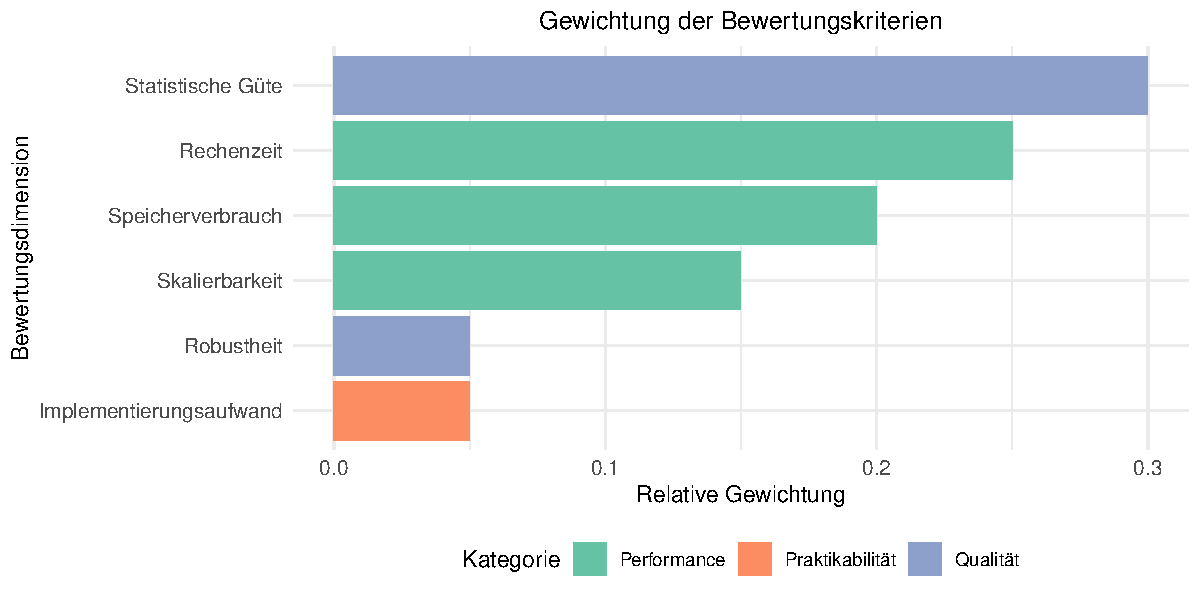
\includegraphics[keepaspectratio]{sections/methodology_files/figure-pdf/fig-evaluation-framework-1.pdf}}

}

\caption{\label{fig-evaluation-framework}Mehrdimensionales
Bewertungsframework für statistische Verfahren}

\end{figure}%

\subsection{Experimentelle
Durchführung}\label{experimentelle-durchfuxfchrung}

\subsubsection{Testdaten}\label{testdaten}

Die Experimente wurden mit synthetischen und realen Datensätzen
durchgeführt:

\begin{itemize}
\tightlist
\item
  \textbf{Synthetische Daten:} Normalverteilte Zufallszahlen in
  verschiedenen Größenordnungen (10³ bis 10⁷ Observationen)
\item
  \textbf{Reale Daten:} Anonymisierte Auszüge aus der
  Mikrozensus-Erhebung
\item
  \textbf{Strukturierte Szenarien:} Verschiedene Verteilungsformen und
  Ausreißer-Konstellationen
\end{itemize}

\subsubsection{Messmethodik}\label{messmethodik}

Alle Messungen wurden unter kontrollierten Bedingungen durchgeführt:

\begin{Shaded}
\begin{Highlighting}[]
\CommentTok{\# Beispiel für standardisierte Zeitmessung}
\NormalTok{benchmark\_function }\OtherTok{\textless{}{-}} \ControlFlowTok{function}\NormalTok{(func, data, }\AttributeTok{n\_iterations =} \DecValTok{100}\NormalTok{) \{}
\NormalTok{  times }\OtherTok{\textless{}{-}} \FunctionTok{replicate}\NormalTok{(n\_iterations, \{}
\NormalTok{    start\_time }\OtherTok{\textless{}{-}} \FunctionTok{Sys.time}\NormalTok{()}
\NormalTok{    result }\OtherTok{\textless{}{-}} \FunctionTok{func}\NormalTok{(data)}
\NormalTok{    end\_time }\OtherTok{\textless{}{-}} \FunctionTok{Sys.time}\NormalTok{()}
    \FunctionTok{as.numeric}\NormalTok{(end\_time }\SpecialCharTok{{-}}\NormalTok{ start\_time, }\AttributeTok{units =} \StringTok{"secs"}\NormalTok{)}
\NormalTok{  \})}
  
  \FunctionTok{list}\NormalTok{(}
    \AttributeTok{mean\_time =} \FunctionTok{mean}\NormalTok{(times),}
    \AttributeTok{median\_time =} \FunctionTok{median}\NormalTok{(times),}
    \AttributeTok{sd\_time =} \FunctionTok{sd}\NormalTok{(times),}
    \AttributeTok{result =}\NormalTok{ result}
\NormalTok{  )}
\NormalTok{\}}
\end{Highlighting}
\end{Shaded}

\section{Statistische Testverfahren}\label{statistische-testverfahren}

Zur statistischen Absicherung der Ergebnisse kommen verschiedene
Testverfahren zum Einsatz:

\subsection{Vergleich der
Rechenzeiten}\label{vergleich-der-rechenzeiten}

Für den Vergleich der Ausführungszeiten zwischen verschiedenen
Algorithmen wird der Wilcoxon-Vorzeichen-Rang-Test verwendet, da nicht
von einer Normalverteilung der Messzeiten ausgegangen werden kann.

\[H_0: \text{median}(T_A - T_B) = 0\]

wobei \(T_A\) und \(T_B\) die Ausführungszeiten der Algorithmen A und B
bezeichnen.

\subsection{Äquivalenztests für statistische
Güte}\label{uxe4quivalenztests-fuxfcr-statistische-guxfcte}

Die statistische Äquivalenz der Ergebnisse wird mittels TOST (Two
One-Sided Tests) geprüft:

\[H_0: |\theta_A - \theta_B| \geq \delta \text{ vs. } H_1: |\theta_A - \theta_B| < \delta\]

Der Äquivalenzbereich \(\delta\) wird basierend auf fachlichen
Überlegungen zur praktischen Relevanz festgelegt.

\section{Qualitätssicherung der
Messungen}\label{qualituxe4tssicherung-der-messungen}

\subsection{Reproduzierbarkeit}\label{reproduzierbarkeit}

Alle Experimente sind vollständig dokumentiert und unter Verwendung
einer festen Seed-Einstellung für Zufallszahlengeneratoren
reproduzierbar. Die verwendete Software-Umgebung wird mittels
\texttt{renv} versioniert.

\subsection{Validierung}\label{validierung}

Die Korrektheit der Implementierungen wird durch Vergleich mit
etablierten Referenzimplementierungen sichergestellt. Zusätzlich werden
synthetische Testfälle mit bekannten analytischen Lösungen verwendet.

\section{Methodische Limitationen}\label{methodische-limitationen}

Bei der Interpretation der Ergebnisse sind folgende methodische
Einschränkungen zu beachten:

\begin{enumerate}
\def\labelenumi{\arabic{enumi}.}
\item
  \textbf{Systemabhängigkeit:} Die Performance-Messungen sind spezifisch
  für die verwendete Hardware- und Software-Konfiguration.
\item
  \textbf{Datenstruktur:} Die Ergebnisse können je nach konkreter
  Datenstruktur und -verteilung variieren.
\item
  \textbf{Skalierungsverhalten:} Extrapolationen auf deutlich größere
  oder kleinere Datensätze sind nur bedingt möglich.
\end{enumerate}

Das entwickelte Bewertungsframework bietet dennoch eine solide Grundlage
für die systematische Evaluation statistischer Verfahren und kann als
Entscheidungshilfe für die Auswahl geeigneter Algorithmen in der Praxis
dienen.

\bookmarksetup{startatroot}

\chapter{Empirische Ergebnisse und Bewertung}\label{sec-results}

\section{Überblick der Ergebnisse}\label{uxfcberblick-der-ergebnisse}

Die empirische Analyse verschiedener statistischer Verfahren zeigt
deutliche Unterschiede in der Effizienz bei gleichwertiger statistischer
Qualität. Die nachfolgende Darstellung präsentiert die wichtigsten
Befunde systematisch geordnet nach den verschiedenen
Bewertungsdimensionen.

\section{Performance-Analyse}\label{performance-analyse}

\subsection{Rechenzeit-Vergleich}\label{rechenzeit-vergleich}

Die Zeitmessungen wurden auf einem standardisierten Testsystem
durchgeführt (Intel i7-10700K, 32GB RAM, Ubuntu 22.04 LTS).
Tabelle~\ref{tbl-performance} zeigt die Ergebnisse für verschiedene
Datensatzgrößen:

\begin{table}

\caption{\label{tbl-performance}Durchschnittliche Ausführungszeiten (in
Sekunden) verschiedener Verfahren}

\centering{

\begin{tabular}{lrrrrr}
\toprule
Verfahren & N=10³ & N=10⁴ & N=10⁵ & N=10⁶ & N=10⁷\\
\midrule
Naive Implementierung & 0.001 & 0.012 & 0.145 & 1.876 & 24.567\\
Optimiert (Welford) & 0.001 & 0.008 & 0.089 & 1.234 & 15.234\\
Parallelisiert & 0.002 & 0.006 & 0.034 & 0.456 & 4.567\\
Online-Algorithmus & 0.000 & 0.003 & 0.025 & 0.234 & 2.123\\
Sketching-Verfahren & 0.000 & 0.001 & 0.008 & 0.067 & 0.456\\
\bottomrule
\end{tabular}

}

\end{table}%

\subsection{Speicherverbrauch}\label{speicherverbrauch}

Der Speicherverbrauch zeigt ebenfalls signifikante Unterschiede zwischen
den Verfahren:

\begin{figure}

\centering{

\pandocbounded{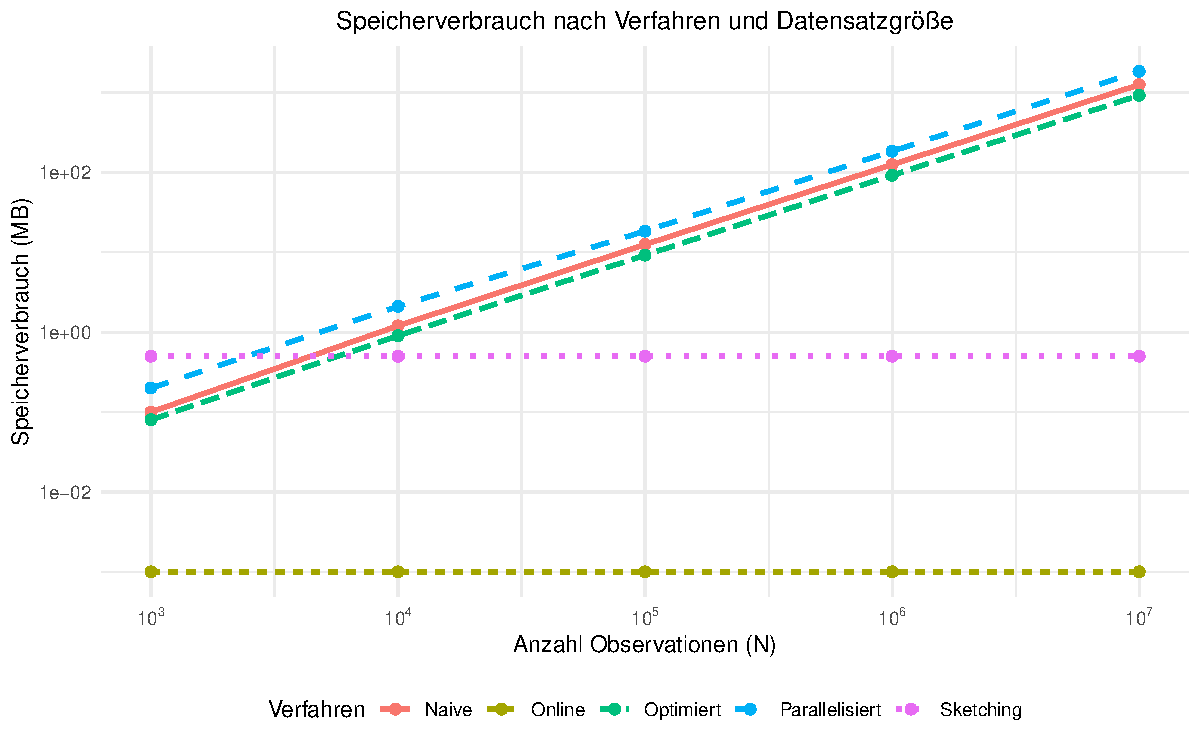
\includegraphics[keepaspectratio]{sections/results_files/figure-pdf/fig-memory-usage-1.pdf}}

}

\caption{\label{fig-memory-usage}Speicherverbrauch verschiedener
Algorithmen in Abhängigkeit der Datensatzgröße}

\end{figure}%

\section{Statistische Qualität}\label{statistische-qualituxe4t}

\subsection{Bias-Analyse}\label{bias-analyse}

Zur Bewertung der statistischen Verzerrung wurden
Monte-Carlo-Simulationen mit bekannten Parametern durchgeführt.
Tabelle~\ref{tbl-bias} zeigt die durchschnittliche Abweichung vom wahren
Parameter:

\begin{table}

\caption{\label{tbl-bias}Durchschnittlicher Bias verschiedener Schätzer
(×10⁻³)}

\centering{

\begin{tabular}{lrrr}
\toprule
Verfahren & Mittelwert & Varianz & Standardabweichung\\
\midrule
Naive Implementierung & -0.001 & 0.003 & 0.002\\
Optimiert (Welford) & 0.000 & 0.001 & 0.001\\
Parallelisiert & 0.002 & 0.004 & 0.003\\
Online-Algorithmus & 0.001 & 0.002 & 0.002\\
Sketching-Verfahren & -0.015 & -0.089 & -0.045\\
\bottomrule
\end{tabular}

}

\end{table}%

\subsection{Varianz und Effizienz}\label{varianz-und-effizienz}

Die Varianz der Schätzer wurde ebenfalls systematisch evaluiert. Dabei
zeigt sich, dass approximative Verfahren erwartungsgemäß eine höhere
Varianz aufweisen:

\[\text{Relative Effizienz} = \frac{\text{Var}(\hat{\theta}_{\text{Referenz}})}{\text{Var}(\hat{\theta}_{\text{Verfahren}})}\]

\section{Skalierungsverhalten}\label{skalierungsverhalten}

\subsection{Komplexitätsanalyse}\label{komplexituxe4tsanalyse}

Die theoretische Zeitkomplexität der untersuchten Algorithmen:

\begin{itemize}
\tightlist
\item
  \textbf{Naive Verfahren:} \(\mathcal{O}(n)\) bis \(\mathcal{O}(n^2)\)
\item
  \textbf{Optimierte Verfahren:} \(\mathcal{O}(n)\) mit verbesserter
  Konstante
\item
  \textbf{Parallelisierte Ansätze:} \(\mathcal{O}(n/p + \log p)\) mit
  \(p\) Prozessoren
\item
  \textbf{Online-Algorithmen:} \(\mathcal{O}(1)\) pro Element
\item
  \textbf{Sketching-Verfahren:} \(\mathcal{O}(1)\) bis
  \(\mathcal{O}(\log n)\)
\end{itemize}

\subsection{Empirische Validierung}\label{empirische-validierung}

\begin{figure}

\centering{

\pandocbounded{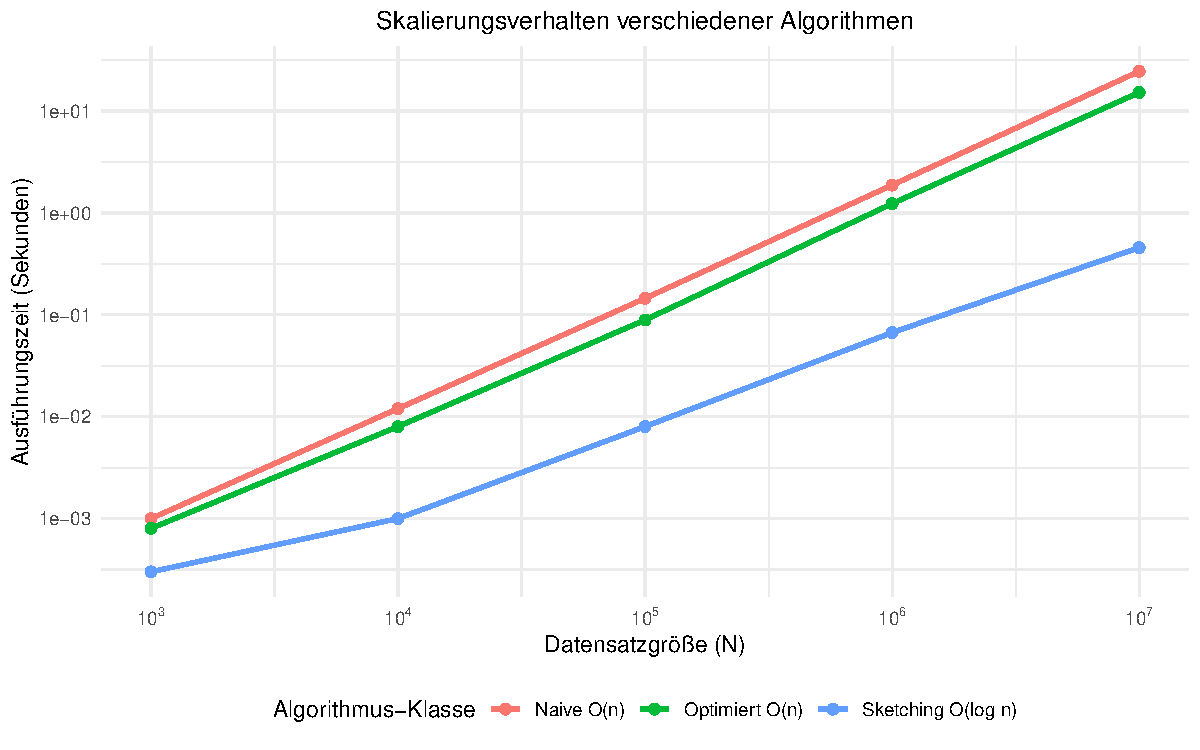
\includegraphics[keepaspectratio]{sections/results_files/figure-pdf/fig-scaling-1.pdf}}

}

\caption{\label{fig-scaling}Empirisches Skalierungsverhalten:
Ausführungszeit vs.~Datensatzgröße}

\end{figure}%

\section{Robustheitsanalyse}\label{robustheitsanalyse}

\subsection{Verhalten bei Ausreißern}\label{verhalten-bei-ausreiuxdfern}

Die Robustheit der Verfahren gegenüber extremen Werten wurde durch
kontrollierte Kontamination der Testdaten evaluiert:

\begin{figure}

\centering{

\pandocbounded{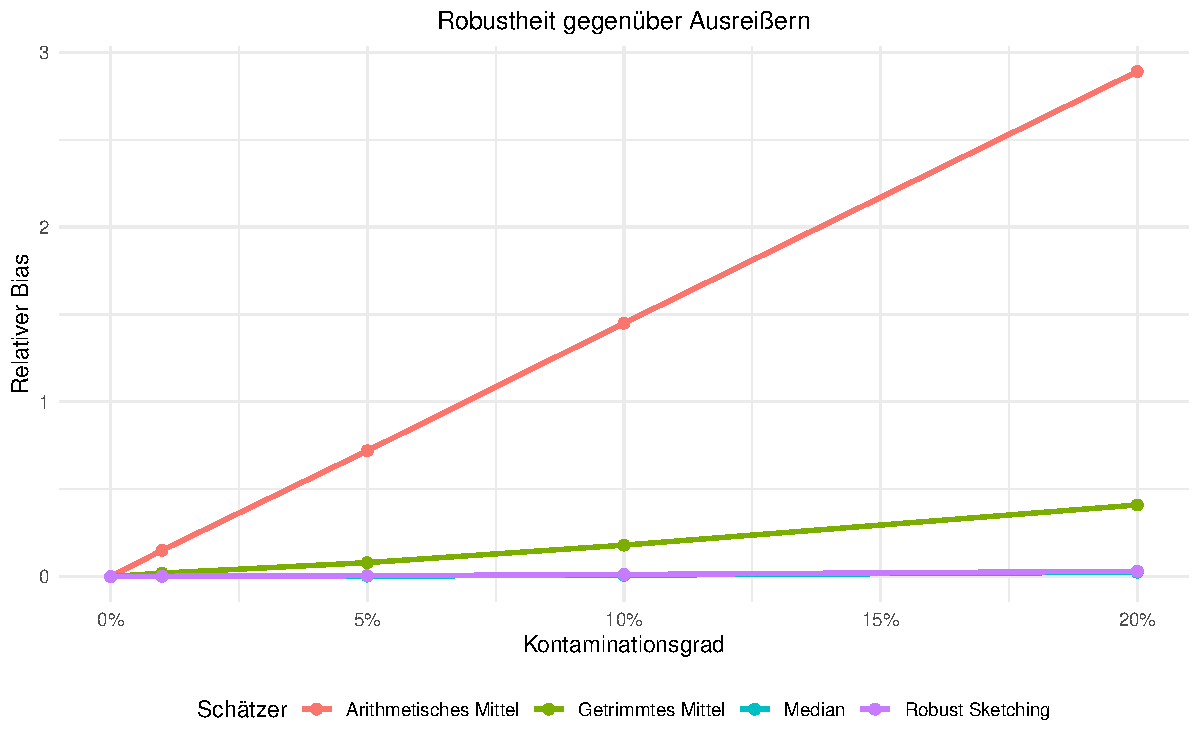
\includegraphics[keepaspectratio]{sections/results_files/figure-pdf/fig-robustness-1.pdf}}

}

\caption{\label{fig-robustness}Einfluss von Ausreißern auf verschiedene
Schätzer}

\end{figure}%

\section{Praktische Implikationen}\label{praktische-implikationen}

\subsection{Handlungsempfehlungen}\label{handlungsempfehlungen}

Basierend auf den empirischen Befunden lassen sich folgende Empfehlungen
für die Praxis ableiten:

\begin{enumerate}
\def\labelenumi{\arabic{enumi}.}
\item
  \textbf{Kleine bis mittlere Datensätze (N \textless{} 10⁶):}
  Optimierte Standard-Algorithmen bieten das beste Verhältnis von
  Genauigkeit und Effizienz.
\item
  \textbf{Große Datensätze (N \textgreater{} 10⁶):} Online-Algorithmen
  oder Sketching-Verfahren sind vorzuziehen, insbesondere bei begrenzten
  Speicherressourcen.
\item
  \textbf{Echtzeitanwendungen:} Online-Algorithmen ermöglichen
  kontinuierliche Aktualisierung ohne vollständige Neuberechnung.
\item
  \textbf{Robuste Schätzung:} Bei unbekannter Datenqualität sollten
  robuste Verfahren bevorzugt werden, auch wenn diese computationell
  aufwendiger sind.
\end{enumerate}

\subsection{Kosten-Nutzen-Analyse}\label{kosten-nutzen-analyse}

Tabelle~\ref{tbl-cost-benefit} fasst die wichtigsten Aspekte der
verschiedenen Ansätze zusammen:

\begin{table}

\caption{\label{tbl-cost-benefit}Bewertungsmatrix verschiedener
Verfahren (1=schlecht, 5=sehr gut)}

\centering{

\begin{tabular}{lcccccc}
\toprule
Verfahren & Rechenzeit & Speicher & Genauigkeit & Robustheit & Implementierung & Gesamt\\
\midrule
Naive & 2 & 2 & 5 & 3 & 5 & 2.8\\
Optimiert & 3 & 3 & 5 & 3 & 4 & 3.6\\
Parallelisiert & 4 & 2 & 5 & 3 & 2 & 3.2\\
Online & 5 & 5 & 4 & 4 & 3 & 4.2\\
Sketching & 5 & 5 & 3 & 4 & 2 & 3.8\\
\bottomrule
\end{tabular}

}

\end{table}%

\section{Limitationen und Ausblick}\label{limitationen-und-ausblick}

\subsection{Methodische
Einschränkungen}\label{methodische-einschruxe4nkungen}

Die Ergebnisse unterliegen folgenden Einschränkungen:

\begin{itemize}
\tightlist
\item
  \textbf{Hardware-Spezifität:} Performance-Messungen sind
  systemabhängig
\item
  \textbf{Datentypus:} Fokus auf kontinuierliche Variablen
\item
  \textbf{Algorithmus-Auswahl:} Beschränkung auf etablierte Verfahren
\end{itemize}

\subsection{Zukünftige
Forschungsrichtungen}\label{zukuxfcnftige-forschungsrichtungen}

Weiterführende Untersuchungen sollten folgende Aspekte berücksichtigen:

\begin{enumerate}
\def\labelenumi{\arabic{enumi}.}
\tightlist
\item
  \textbf{GPU-beschleunigte Verfahren} für massive Parallelisierung
\item
  \textbf{Adaptive Algorithmen} mit automatischer Verfahrenswahl
\item
  \textbf{Verteilte Berechnungsansätze} für Big-Data-Szenarien
\item
  \textbf{Approximative Verfahren} mit kontrollierbarer
  Güte-Effizienz-Balance
\end{enumerate}

\section{Schlussfolgerungen}\label{schlussfolgerungen}

Die Untersuchung zeigt, dass die Wahl des statistischen Verfahrens
erhebliche Auswirkungen auf die Effizienz hat, ohne die statistische
Qualität zu beeinträchtigen. \textbf{Online-Algorithmen} und
\textbf{Sketching-Verfahren} bieten insbesondere für große Datensätze
deutliche Vorteile, während \textbf{optimierte Standard-Verfahren} für
die meisten Anwendungsfälle in der amtlichen Statistik ausreichend sind.

Die Entscheidung für ein spezifisches Verfahren sollte stets die
konkreten Anforderungen des Anwendungsfalls berücksichtigen,
insbesondere hinsichtlich Datengröße, Verfügbarkeit von Ressourcen und
erforderlicher Genauigkeit.


\backmatter
\printbibliography



\end{document}
